\documentclass{article}

% Formatting draft only (pilot subsample). Not camera-ready.
% Filled from stage2_pilot_32b_results.zip (100 trajs, TARGET_TOTAL=100, SEED=0).

\usepackage[utf8]{inputenc}
\usepackage[T1]{fontenc}
\usepackage{hyperref}
\usepackage{url}
\usepackage{booktabs}
\usepackage{amsfonts}
\usepackage{graphicx}
\usepackage{xcolor}

\title{Pilot Results Draft --- Qwen3-32B Value-Axis Transfer\\
\large (100-trajectory subsample; formatting reference)}
\author{}
\date{}

\begin{document}
\maketitle

\noindent\textit{Pilot note.}
These numbers are from a Stage-2 Colab pilot: all 14 successes in the ingested pool plus 86 subsampled failures (100 trajs total), frozen \texttt{value\_axis\_32b.npy}, primary layer 49, thinking ON.
They are \textbf{not} the full verified-200 paper run.
Branches below follow the Results scaffold outcome~\textbf{C} (no frozen-axis transfer), with probes separating (decodability without axis alignment).

\section{Results}
\label{sec:results}

\subsection{Reconstruction and Data Overview}
\label{sec:results-overview}

Our reconstruction of the value axis reproduces the published single-turn separation pattern on Qwen3-32B with thinking enabled: held-out AUROC of $0.872$ at layer 49, with the strongest separation at layers 45--50, consistent with Jiang et al.\ at a lower absolute ceiling than their Qwen3-8B $0.95+$ result.
Layer 49 is fixed as the primary layer for all subsequent analyses.

\begin{figure}[ht]
  \begin{minipage}[b]{0.48\linewidth}
    \centering
    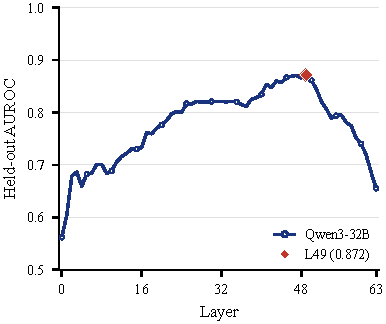
\includegraphics[width=\linewidth]{stage1/data/figures/fig_auroc_by_layer_32b_panel.pdf}
    \small\textbf{(a)} Held-out AUROC by layer.
  \end{minipage}
  \hfill
  \begin{minipage}[b]{0.48\linewidth}
    \centering
    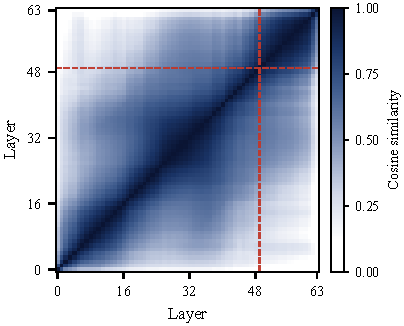
\includegraphics[width=\linewidth]{stage1/data/figures/fig_axis_cosine_32b_panel.pdf}
    \small\textbf{(b)} Pairwise similarity across layers.
  \end{minipage}
  \caption{\textbf{The Qwen3-32B value axis generalizes to held-out ICRL criteria.}
  \textbf{(a)} Held-out AUROC peaks at layer 49 ($0.872$).
  \textbf{(b)} Axis directions are similar in middle-to-late layers; early and late directions are nearly orthogonal.}
  \label{fig:probe_eval_32b}
\end{figure}

\paragraph{Pilot transfer sample.}
From 198 ingested verified trajectories (14 resolved / 184 unresolved), we keep \textbf{all 14 successes} and randomly subsample failures to a pilot of \textbf{100} trajectories (14 resolved, 86 unresolved; majority-class baseline $0.86$).
Exit statuses in the pilot: 97 \texttt{Submitted}, 3 \texttt{LimitsExceeded}.
Trajectory lengths range from 4 to 59 steps (median 8, mean 12.3); resolved trajectories are shorter (median 7) than unresolved ones (median 8), and all trajectories with $>20$ steps are unresolved ($n{=}17$).
Because this is a one-seed design, no task has mixed outcomes across seeds ($0$ mixed-outcome tasks).

%% FIG (appendix candidate): length histogram by outcome --- useful here
%% because length asymmetry / long-failure confound matters for probes.

\subsection{Final-Step Transfer}
\label{sec:results-final}

At the final step, the frozen axis \textbf{does not separate} outcomes: AUROC $0.488$ $[0.326,\ 0.651]$ against a majority-class baseline of $0.860$, with the interval including chance ($0.5$).
The task-level permutation test yields $p = 0.885$.
The final-token robustness readout gives AUROC $0.492$, consistent with the token-mean readout.
Class means of \texttt{proj\_mean} are essentially identical (unresolved $0.1345$ vs.\ resolved $0.1334$); the final-step histograms fully overlap (Figure~\ref{fig:final_step_pilot}).

\begin{figure}[ht]
  \centering
  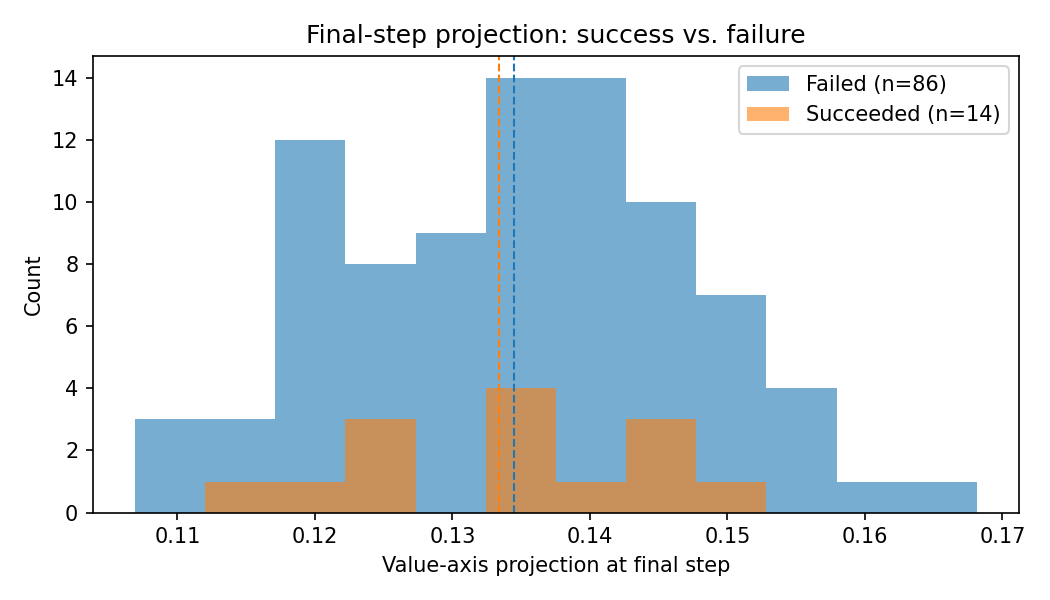
\includegraphics[width=0.72\linewidth]{_pilot_analysis/analysis_report_pilot/final_step_separation.png}
  \caption{\textbf{Pilot: the frozen axis does not separate outcomes at the final step.}
  Layer-49 mean-over-$G_t$ projections for resolved ($n{=}14$) vs.\ unresolved ($n{=}86$) trajectories.}
  \label{fig:final_step_pilot}
\end{figure}

\subsection{Trajectory Evolution}
\label{sec:results-evolution}

Across relative-position bins, the frozen axis does \textbf{not} show the late-emerging transfer pattern hypothesized for a transferring value signal.
Per-bin AUROCs (layer 49) are
$0.339$ $[0.247,\ 0.442]$ (early),
$0.265$ $[0.185,\ 0.385]$,
$0.367$ $[0.182,\ 0.535]$,
$0.457$ $[0.283,\ 0.622]$,
and $0.492$ $[0.350,\ 0.644]$ (late).
Early bins show \emph{inverted} separation (AUROC $\ll 0.5$, CIs entirely below chance); mid-to-late bins approach chance with intervals that include $0.5$.
Late-bin separation-to-noise is $0.023$.
Readout-noise check: \texttt{proj\_mean} std $0.015$ $<$ \texttt{proj\_final} std $0.025$, as expected for averaging over $G_t$.

%% FIG (MAIN for paper; pilot uses table/numbers above):
%% per-bin AUROC vs rel\_pos with CI bands.

\subsection{Layer Localization}
\label{sec:results-layers}

Fixing the primary layer is not the sole explanation for the null.
A final-step sweep over all 64 layers yields AUROCs mostly near chance in the ``correct'' direction; the maximum above $0.5$ is only $0.615$ (layer 44), and several late layers are strongly \emph{anti}-aligned with success (e.g.\ layer 59 AUROC $0.292$).
Layer 49 (pre-registered from ICRL) sits at $0.488$.
We do \textbf{not} interpret inverted late-layer AUROCs as a transferring value signal without a pre-registered flip and held-out confirmation.
Held-out trajectory re-selection for layer choice was not run in this pilot.

%% FIG (appendix/main): final-step AUROC vs layer, ICRL curve optional overlay.

\subsection{Internal Signal versus Verbalized Confidence}
\label{sec:results-elicited}

\textbf{Not run in this pilot.}
Stage-4 post-hoc elicitation (verbalized $P(\mathrm{success})$) was deferred.
Under outcome~C for the frozen axis, this comparison is secondary; we will report it for completeness on the full run if budget allows.
\textit{Scaffold branch C (placeholder):} Neither signal separates outcomes until elicitation exists; the comparison is currently uninformative for the internal axis alone.

\subsection{Fitted-Probe Reference}
\label{sec:results-probes}

Fitted $\ell_2$ logistic probes under task-level 5-fold CV achieve a grid-max AUROC of $0.935$ at layer 51, relative-position bin 3 ($0.7$), and a \textbf{grid-mean} AUROC of $0.748$ across all $64{\times}5$ cells (all cells used 5 folds).
At the primary layer 49, bin-wise probe AUROCs are $0.769$, $0.804$, $0.725$, $0.794$, and $0.834$ (late bin).
The full layer-by-position grid is in the pilot CSV (\texttt{probe\_auroc\_grid.csv}).

\textbf{Branch C / probes DO separate:}
Fitted probes separate outcomes where the frozen axis does not.
Outcome information is present in agentic mean-pooled residuals but not along the original ICRL value axis --- the representation, not the information, fails to transfer on this pilot.
We treat \texttt{grid\_max} as a summary only (selection over the layer$\times$bin family can overfit); the elevated \emph{mean} across the grid is the more informative decodability signal.
Caveat: with only 14 successes, and with trajectory length correlated with failure, probe AUROCs may partly reflect length or other correlates; confound checks are required before a paper claim.

\begin{table}[ht]
  \centering
  \begin{tabular}{lcc}
    \toprule
     & Frozen axis (L49) & Fitted probes \\
    \midrule
    Final / late readout AUROC
      & $0.488$ $[0.326,\ 0.651]$
      & $0.834$ (L49, late bin; CV mean) \\
    Best cell (summary only)
      & ---
      & $0.935$ (L51, bin 3) \\
    Grid mean (all layers $\times$ bins)
      & ---
      & $0.748$ \\
    Permutation $p$ (final-step axis)
      & $0.885$
      & --- \\
    \bottomrule
  \end{tabular}
  \caption{\textbf{Pilot four-way summary:} frozen axis null, fitted probes decodable
  (outcome information present; not aligned with the ICRL axis).}
  \label{tab:frozen_vs_fitted_pilot}
\end{table}

\subsection{Within-Task Contrast}
\label{sec:results-within}

Restricting to mixed-outcome tasks is \textbf{not applicable} in this one-seed pilot: $0$ tasks have both resolved and unresolved rollouts.
The within-task gap is undefined (\texttt{within\_task\_n\_mixed}${}=0$).
This contrast requires multi-seed data or a different design; we omit it rather than over-interpret the pooled null.

% =====================================================================
% PILOT NOTES (delete / rewrite for paper):
% - Design is 100 = 14 succ + 86 fail from verified ingest, not 60x5.
% - Model is Qwen3-32B (not 8B); thinking ON.
% - Elicitation skipped; probes + frozen axis are the pilot punchline.
% - Do not claim population null; CI still wide; n_success=14.
% =====================================================================

\end{document}
